\documentclass{article}
\usepackage{graphicx} % Required for inserting images
\usepackage[margin=1in]{geometry}
\usepackage{url}
\usepackage{hyperref}

\usepackage{float}
\usepackage{amsmath}


\title{CS310 Progress Report: Evaluating the Performance of Blink Detection on DeepFakes Injected With Adversarial Noise}
\author{Joel Coulon, 2204489}
\date{}

\begin{document}

\maketitle

\section{Project Introduction}

A DeepFake refers a video of an individual is digitally altered or created by an Artificial Intelligence (AI). These are often generated using Generative Adversarial Network (GANs) models and are trained via the adversarial of two models: one attempting to generate a realistic image, the other attempting to detect the inaccuracies. These two then train each other until the original model can generate videos that are deemed realistic by the detector.\\

Initially, these models were fairly obvious to detect, even for humans, for example see Figure \ref{fig:earlyexample}. Various features, such as temporal inconsistencies, feature irregularities, and inconsistencies in lighting produced by GANs were all tell-tale signs of DeepFaked imagery. However, over time, GANs have developed resulting in DeepFakes now being almost impossible to tell apart from genuine videos by humans.

\begin{figure}[H]
    \centering
    \fbox{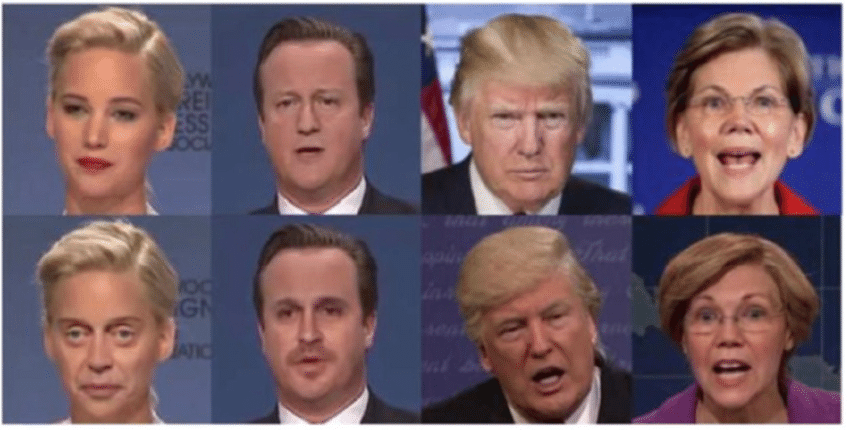
\includegraphics[width=0.5\linewidth]{images/Examples-of-original-and-deepfake-videos.png}}
    \caption{An early of example of DeepFakes with original images on the top, faked images on the bottom\cite{earlydeepfakeimage}}
    \label{fig:earlyexample}
\end{figure}

Due to their difficulty to be accurately identified by humans, DeepFakes soon became a popular way to spread misinformation by faking an individual's likeness. For example, DeepFakes were used by a variety of sources to promote political parties in the 2021 Lebanese elections\cite{misinformation}. The other primary use of DeepFakes is pornography with an estimated 98\% of DeepFakes being porn\cite{pornography}, including the first main-stream DeepFake in 2017 of actress Gal Gadot\cite{misinformation}.\\

Ever since the creation of DeepFakes there has been efforts to detect them. Original DeepFake detection methods relied on pixel analysis and visual artifacts present in early DeepFakes\cite{yu2021survey}. However through a combination of improvement in generation techniques and adversarial noise attacks\cite{huang2020fakeretouch}\cite{pertubations}, these original methods are proving increasingly ineffective.\\

One method proposed to tackle modern DeepFakes is blink detection. Blinking is a subconscious act for humans and falls into a predictable patterns. DeepFakes are notoriously bad at simulating blinking, either by not blinking at all or blinking in unnatural intervals. Thus methods have been used to leverage these temporal inconsistencies to detect DeepFakes with a high degree of accuracy\cite{blinking-pattern}.\\

So far, the resilience of blink-detection to adversarial noise has not been studied. It seems likely that due to this method relying on identification of features rather than individual pixels, it seems likely that adversarial noise would not affect the detection of a DeepFake in any meaningful way. This project aims to verify whether this assumption is true or not.

\section{Literature Review}

This project combines two thoroughly-research topics (Blink-based DeepFake detection and Adversarial noise injection) which have had extensive research on both of them.

\subsection{Blink Detection}
\subsubsection{DeepVision}

DeepVision\cite{blinking-pattern} is a model that takes into account the time, activity, gender and age of the individual in a video to determine whether a video is DeepFaked or not by comparing their blink patterns to a database of known ``good" blink frequencies\\

The pre-process stage of the model involves categorising the video based on 4 landmarks. The landmarks are: gender, age (in 6 sub-categories varying from \textless 20 to 65+), activity (dynamic or static), and time (am/pm). The frequency of a human varies based on all these features\cite{varying-blink}, and therefore they believe all of these factors need to be taken into account for an accurate detection.\\

To actually detect a blink, two algorithms are used. The first is an algorithm called Fast-HyperFace\cite{ranjan2017hyperface} which is used to detect the landmarks of the face, pose, and gender of the individual in a video. The key landmarks from this are then extracted to then aid in the performance of the second model: Eye-Aspect Ration (EAR). EAR uses 6 points to calculate the absolute area of the horizontal versus the vertical axis to determine if a blink has occurred\cite{EAR}.
\begin{equation}
    EAR=\frac{||p_2-p_6||+||p_3-p_5||}{2||p_1-p_4||}
\end{equation}
The average of the left eye ($EAR_l$) and the right ($EAR_r$) can then be taken to get the mean eye ration ($EAR_i$)
\begin{equation}
    EAR_i = \frac{EAR_l + EAR_r}{2}
\end{equation}
\begin{figure}[H]
    \centering
    \fbox{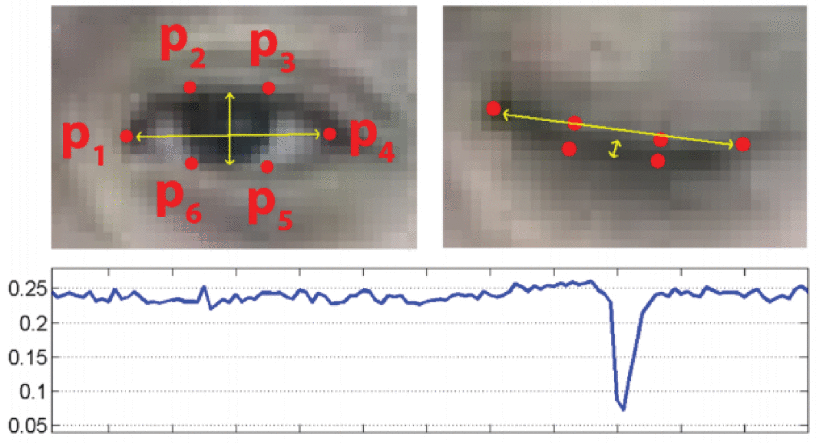
\includegraphics[width=0.5\linewidth]{images/EAR.png}}
    \caption{The EAR algorithm at work with eye landmarks $p_{1-6}$ labelled and a graph representing EAR (y-axis) over time (x-axis)}
    \label{fig:EAR}
\end{figure}

A blink is defined as when $EAR_i$ drops below a certain threshold for multiple consecutive frames. Data such as when the blink occurred in time, the period of blink, and frequency are all extracted and fed into the next stage.\\

This data is then compared with data from a pre-existing database of valid blinks derived from the Eye Blinking Prediction dataset from Kaggle\cite{eyeblinkprediction}. The factors mentioned above are all compared to see how similar they are to valid blinks in authentic videos and if it is within a certain threshold the video is deemed real. The paper does not mention this threshold. \\

DeepVision achieves an overall accuracy of 87.5\%\cite{blinking-pattern}.

\subsubsection{Ictu Oculi}

Ictu Oculi is a secondary method for blink detection, but rather than relying on an existing database for comparison, uses a trained neural network\cite{ictuoculi}.\\

An initial pre-processing step is done to identify the facial landmarks of the image and distort and crop it so that the face is: in the centre of the image; rotated such tat eyes form a horizontal line; and scaled to a similar size across the length of the video.\\

Once pre-processing is complete, the cropped video is sent to a Long-term Recurrent Convolution Neural Network (LRCN). This is three-stage neural network as shown in Figure \ref{fig:LRCN}. 

\begin{figure}[H]
    \centering
    \fbox{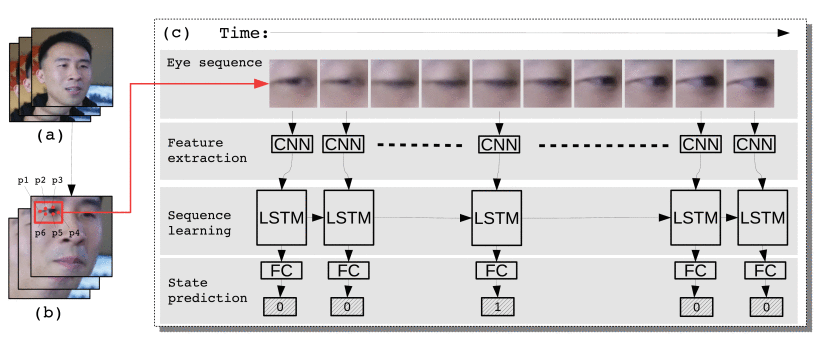
\includegraphics[width=0.75\linewidth]{images/LRCN.png}}
    \caption{Overview of the LRCN method. (a) is the original sequence. (b) is the sequence after face alignment. We crop out eye region of each frame based on eye landmarks $p_1-6$ in (b) and pass it to (c) LRCN, which consists of three parts: feature extraction, sequence learning and state prediction\cite{ictuoculi}}
    \label{fig:LRCN}
\end{figure}

The first part is a typical Convolution Neural Network (CNN) used to extract the discriminative features from the eye region. The next stage is to use a Recursive Neural Network with Long Short Term cells (LSTM-RNN) to guess the probability of eye being in range $[0,1]$ with $0$ equating to eye being open, and $1$ being eye is closed. To do this it uses the following function:

\begin{equation}\begin{array} { l } { f _ { t } = \sigma \left(W _ { f h } h _ { t - 1 } + W _ { f x } x _ { t } + b _ { f } \right) } \\ { i _ { t } = \sigma \left(W _ { i h } h _ { t - 1 } + W _ { i x } x _ { t } + b _ { i } \right) } \\ { g _ { t } = \tanh \left(W _ { c h } h _ { t - 1 } + W _ { c x } x _ { t } + b _ { c } \right) } \\ { C _ { t } = f _ { t } \odot C _ { t - 1 } + i _ { t } \odot g _ { t } } \\ { o _ { t } = \sigma \left(W _ { o h } h _ { t - 1 } + W _ { o x } x _ { t } + b _ { o } \right) } \\ { h _ { t } = o _ { t } \odot \tanh \left(C _ { t } \right) } \end{array}\end{equation}

$\sigma$ is the sigmoid function, $f_t$ is forget gate to control what previous memories will be discard, it is input gate to selectively pass the current input, which is manipulated by $g_t$. $o_t$ is output gate to control how much memory will be transferred into hidden state $h_t$. Memory cell $C_t$ is combined by previous memory cell $C_{t-1}$ controlled by $f_t$ and manipulated input $g_t$ controlled by $i_t$. 256 hidden units are used in the LSTM cell, which is the dimension of LSTM output $z_t$\cite{ictuoculi}. A diagram of such a cell is shown in Figure \ref{fig:LSTM}.

\begin{figure}[H]
    \centering
    \fbox{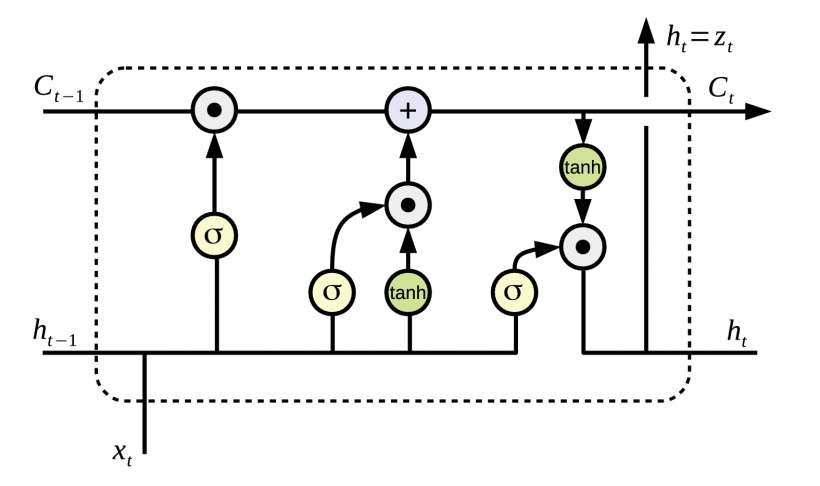
\includegraphics[width=0.5\linewidth]{images/LSTN.png}}
    \caption{A diagram of LSTM structure\cite{ictuoculi}}
    \label{fig:LSTM}
\end{figure}

Finally, the output is then used to determine whether or not a blink has occurred, and over what time period.\\

A simplified method is used to determine whether the blink patterns are consistent with a normal human being. This solely detects the number of blinks in a set period of time (60 seconds),the average person blinks 34.1 times a minute. This leads to an accuracy of 99\% when tested on a dataset of 32 videos.

\subsubsection{Analysis}

DeepVision's primary advantage is that it is very easy to compute and implement. Fast-HyperFace is a pre-trained model and therefore is a simple drag and drop implementation. Once $p_{1-6}$ are located in a frame, it is a simple calculation to determine the $EAR$. The following statistical analysis to determine if the blinking is consistent with real videos or not is also relatively simple and non-computationally intensive. Therefore any methodology involving DeepVision would be fast to implement and relatively easy to debug.\\

The primary downsides to DeepVision is potential obstruction of the eyes. $EAR$ requires the entire eye to be visible in the frame of a video to identify all of the points required. A partial $EAR$ can be calculated with a single eye but the accuracy of this is going to be less than if two eyes were visible. The second disadvantage is the database required to determine whether blinking is consistent with normal blinking. The database requires a large number of labelled examples which would be time consuming to produce.\\

Ictu Oculi has a much more complex blink-detection system, requiring two separate machine learning models to be trained to identify if a blink is happening or not. This is a lot more complex and requires pre-processing resulting in a longer development time and training time. On the other hand, it results in a much more resilient blink detection mechanism as the eyes can be partially obscured in a frame but the eye's state can still be accurately determined.\\

The drawback is that the state of the eye is binary open or close, any information relating to the speed of the blink is lost resulting in a very rudimentary system to determine whether a sequence of blinks is a DeepFake or not. This seems to have little to no effect on accuracy of detection.\\

The planned implementation can be found in Section \ref{sec:future_blink}.

\subsection{Adversarial Noise}



\subsection{Datasets}
\subsection{Noise Reduction}

\section{Current Progress}

\section{Future Progress}
\subsection{Blink Detection} \label{sec:future_blink}

The primary disadvantage of the $EAR$ is that it cannot calculate the state of an eye if any of $p_{1-6}$ is obscured\cite{ictuoculi}. However, various AI models such as Google's MediaPipe \cite{mediapipe} and OpenFace\cite{openface} maintain detection of these features even when obscured. Hence it is possible to maintain an accurate $EAR$ even when the face is partially obscured in a frame. Therefore, for the blink detection in my project, I will initially use MediaPipe as a proof of concept and then move on to training my own model from various eye datasets such as Kaggle's eye blinking prediction\cite{eyeblinkprediction}.\\

Having the $EAR$ data allows for more sophisticated methods of blink detection than what was utilised than Ictu Oculi. However a method such as the database employed by DeepVision\cite{blinking-pattern} would be too time consuming to label and store all the data given the amount of time given to this project. Given the large amount of data available: such as the time taken to blink, the period between blinking, and the overall progression of the $EAR$ it may be possible to train a classifier neural network to determine whether or not a sequence of $EAR$ readings overtime is a that of a genuine video or a DeepFake. As this has never been done before, further research and experimentation would need to be done. For a proof of concept, Ictu Oculi has proved even a simple approach of frequency of blinks is sufficient\cite{ictuoculi}.

\section{Appraisals \& Reflections}

\section{Legal, Social, Ethical, and Professional Issues \& Considerations}

\section{Project Management}

\bibliographystyle{IEEEtran}
\bibliography{progress}

\end{document}